%!TEX root = main.tex
\section{The Sensemaking Model for VQSs\label{sec:sensemaking}}
\change{
  To convey how the features in \zvpp addresses the analytical needs posed by each domain, we organize our PD findings into a sensemaking framework for VQSs. In this section, we first describe the space of problems addressable by VQSs. Then, as shown in Figure~\ref{fig:taxonomy}, we develop a taxonomy for organizing VQS functionalities into three sensemaking processes. From top to bottom, we first describe the design objectives of each sensemaking process, then we outline the design challenge addressed by each of the functional components that supports the sensemaking process. The mapping between specific \zvpp features and these functional components and sensemaking processes can be found in Table~\ref{bigfeaturetable}.
}
 %Starting from the bottom level of the taxonomy, we first describe what each component in our taxonomy encompasses, then we proceed onto the upper level of the taxonomy, .
%We first describe features that we incorporated into our enhanced VQS, \zvpp, thematically organized by components (grouping features in the bottom-most level to components in the second level of Figure~\ref{fig:taxonomy}).
%collaboratively-designed
%Next, we describe features that we incorporated into our enhanced VQS, \zvpp, thematically organized by component. Then, we introduce a taxonomy for organizing these components into three sensemaking processes, spanning different problem areas that VQSs are aimed to solve.
%\change{In this section, we will first introduce a taxonomy for organizing these components into}
%Based on feature requests and discussion with our participants, we incorporated key features missing in our original VQS.
%From these discussion and analysis of past VQSs, we identify nine components of VQSs, described below. T
% Along with analysis of past literature, we develop a taxonomy of key functionalities in VQSs.
% novel contribution on  ---
% contribute to holistic understanding on how sensemaking --- in VQS.
% study on how users
% Implication ---
% •	What types of questions/ dataset/ problem challenges are asked to VQS or can be addressed by VQS? (S3)
% •	What kind of features needs to be designed to address these challenges (S4 PD)
%We employed participatory design with our scientists to incorporate key features missing in our original VQS, and unaddressed in their existing workflows. From these discussion and analysis of past VQSs, we identify nine components of VQSs, described below.
\subsection{Characterizing the Problem Space for VQSs}
%Based on example use cases and feature components from participatory design, we further characterize the design space of VQSs. further characterize three sensemaking process within the problem space of VQSs.
Given our earlier description of VQS features organized into components, we now introduce the three sensemaking processes by characterizing how they fit into different problem areas that VQSs are aimed to solve. Visual querying often consists of searching for a desired pattern instance (Z) across a visualization collection specified by some given attributes (X,Y). \change{Correspondingly, }we introduce two axes depicting the amount of information known about the visualized attribute and pattern instance.%, as shown in Figure~\ref{2dmodel}.
%(e.g., only interested in patterns related to a specific gene)
\par Along the \textbf{pattern instance} axis,
the visualization that contains
the desired pattern may already be \texttt{known} to the analyst,
exist as a pattern \texttt{in-the-head} of the analyst,
or completely \texttt{unknown} to the analyst.
In the \texttt{known} pattern instance region (Figure~\ref{2dmodel} grey), visualization-at-a-time systems such as Tableau,
where analyst manually create and examine each visualization one at a time,
is more well-suited than VQSs, since analysts can directly work with the selected instance without the need for visual querying.
Inspired by Pirolli and Card's information
foraging framework~\cite{Pirolli}, which distinguishes
between information processing tasks that are \textit{top-down}
(from theory to data) and \textit{bottom-up} (from data to theory),
we define \textit{top-down pattern specification} as the search-oriented paradigm where analysts query based on their
in-the-head pattern (Figure~\ref{2dmodel} blue) in a fixed collection.
On the other hand, in the realm of \textit{bottom-up
data-driven inquiry} (Figure~\ref{2dmodel} green),
the pattern of interest is unknown\change{, external
to the user, }and must be driven by recommendations
or queries that originate from the data (or equivalently, the visualization).
As we will discuss later, this process is crucial
but underexplored in past work on VQSs.
%analysts often do not start with a known pattern instance. T
\par The second axis, \textbf{visualized attributes},
depicts how much the analyst
knows about which X and Y axes
they are interested in visualizing.
In both the astronomy and genetics use cases,
as well as past work in this space,
data was in the form of a time series
with \texttt{known} visualized attributes.
In the case of our material science participants,
they wanted to explore relationships between different
X and Y variables.
In this realm of \texttt{unknown} attributes,
context creation (Figure~\ref{2dmodel} yellow) is
essential for allowing users
to pivot across different visualization collections.%subspaces. %Most past VQSs assume that the analyst has a desired pattern in-the-head that could be conveyed through visual specification, such as a sketch.%---i.e., setting the stage for bottom-up or top-down processes---\dor{this clause is awkward?}
\begin{figure}[h!]
  \centering
  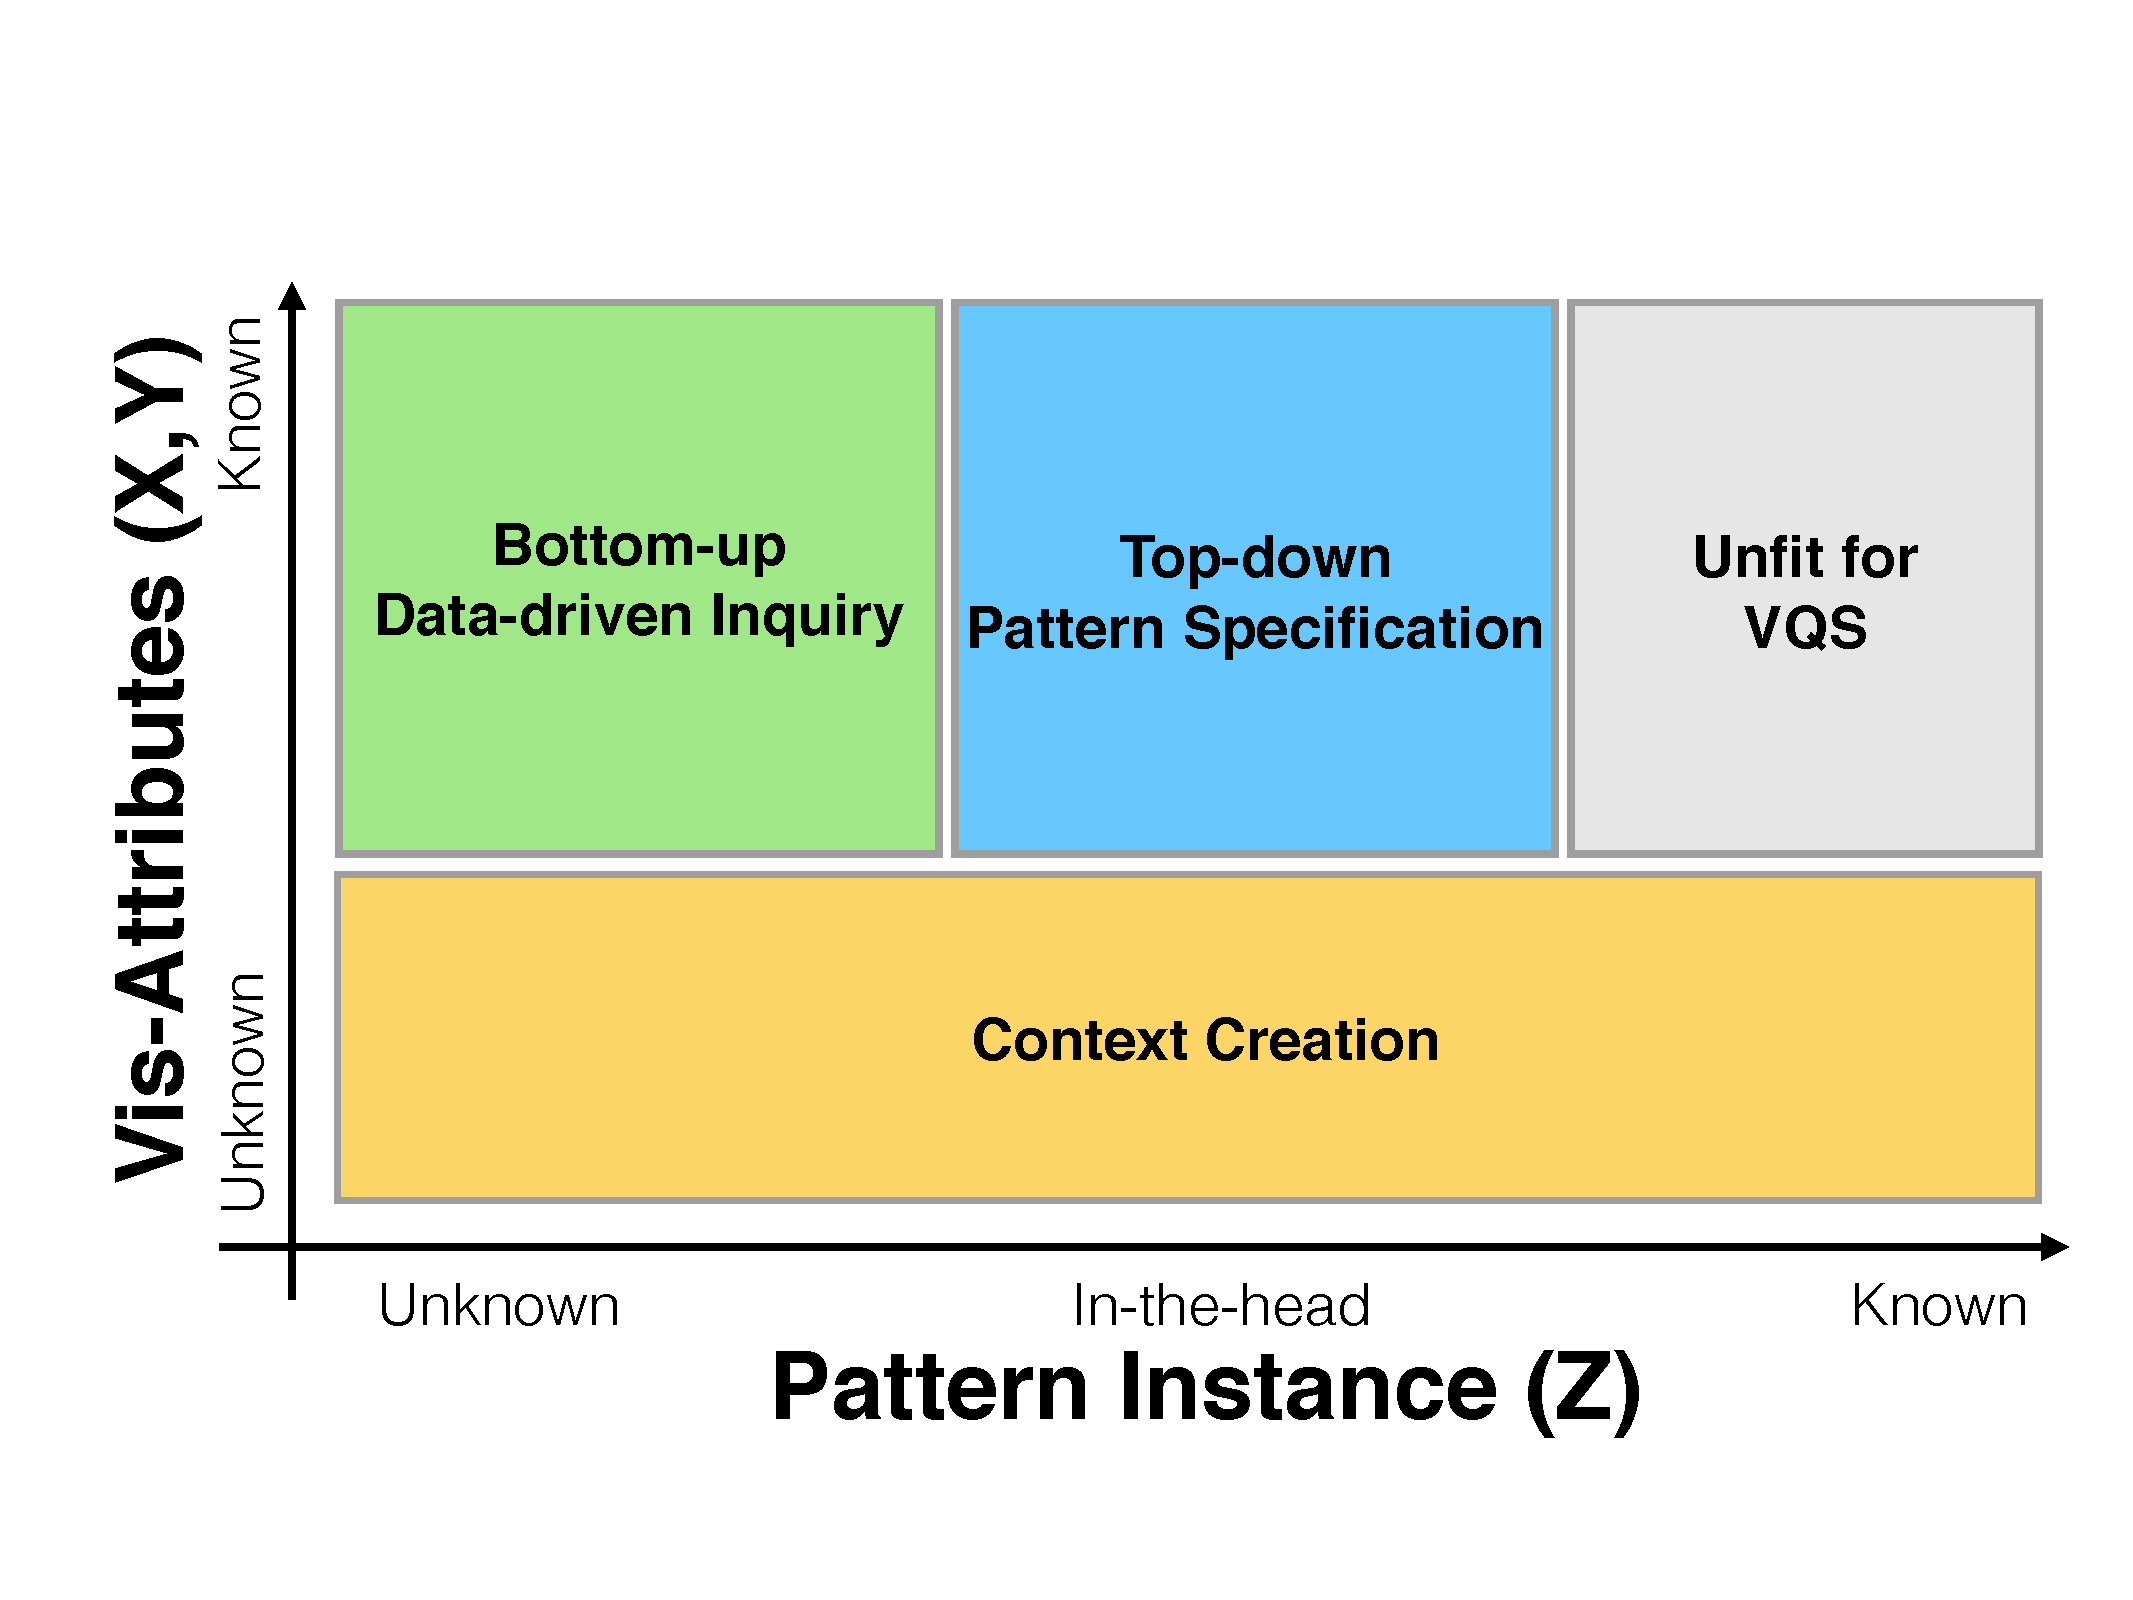
\includegraphics[width=0.9\linewidth]{figures/2dmodel.pdf}
  \caption{The problem space for VQSs is characterized by how much the analyst knows about the visualized attributes and the pattern instance. Colored areas highlight the three sensemaking processes in VQSs for addressing these characteristic problems. While prior work has focused solely on use cases in the blue region, we envision opportunities for VQSs beyond this to a larger space of use cases covered by the yellow and green regions.}
  \label{2dmodel}
  \vspace{-10pt}
\end{figure}
\subsection{Design Goals for the Sensemaking Processes}
After understanding how each sensemaking process fits into the problem space \change{addressable} by VQSs, we further explore the design objectives and challenges in supporting each sensemaking process, grounded in our collaborative design experience. % based on the taxonomy orgaby developing a taxonomy for organizing the aforementioned components.% fits into the paradigms of sensemaking in VQSs, as shown in Figure~\ref{fig:taxonomy}. In particular, we will describe the main form of inquiry addressed by each paradigm\cut{(\textit{what, where, which})}, its characteristic use case, and design challenges in supporting these paradigms.
% \par Drawing from our participatory design experience, evaluation study, and literature review in this space, we design a taxonomy for understanding the key functionalities in VQSs. In Figure~\ref{fig:taxonomy}, we show how each use cases makes use of the different features in \zv, then we organize the features into key components for VQSs, which belongs to one of the three paradigms in the VQS design space.%, effectively moving rightwards to the gray area in Figure~\ref{2dmodel}, where the pattern instance is known.
\boldpara{Top-down Pattern Specification} begins with the user's intuition
about how their desired patterns should look like based on `theory', including visualizations from past experience or abstract conceptions based on external knowledge. The goal of top-down pattern specification is to address the \textit{which} question of visual sensemaking: \textit{which pattern instance exhibits this pattern?} Based on this preconceived notion of what to search for, the design challenge is to translate the query in the
analyst's head to a query executable by the VQS.
\change{In the Figure~\ref{fig:taxonomy} taxonomy},
this includes both components for specifying the pattern,
as well as controls governing the underlying
algorithm of how shape-matching is performed.
For example, A1 knows intuitively
what a supernovae pattern looks like
and the detailed constraints on the shape,
such as the width and height of the peak
or the level of error tolerance for defining a match.
He can search for transient patterns through sketching,
select the option to ignore differences
on the x axis, and changes the similarity metric for flexible matching.  %The design challenge of top-down pattern specification is to ----- enable users to How to translate the in-the-head query to visual query and how matching is done.
\boldpara{Bottom-up data-driven inquiry} is
a browsing-oriented sensemaking process
that goes from data to theory to
addresses the \textit{what} questions
in the sensemaking process.
% While the usage of each querying feature may vary from one participant to the next, generally, result querying and pattern upload are considered bottom-up approaches that go from data to theory by enabling users to query via examples of known visualizations. Bottom-up data-driven inquiries
 For example, genetics participants do not
 have a preconceived knowledge of what to search
 for in the dataset.
 They were mostly interested in
 \textit{what types of patterns exist in the dataset}
 through representative trends, as a means to
 jumpstart further queries. %The goal of data-driven inquiry is to move towards the blue area in Figure~\ref{2dmodel} to help analysts gain more information about patterns of interest in-the-head.
% notion of what the pattern looks like
The design challenge include developing
the right set of `stimuli' that could
provoke further data-driven inquiries,
as well as low-effort mechanisms to search via these results.
\boldpara{Context Creation} addresses the \textit{where}
question of sensemaking by enabling analysts
to navigate across different parts of the visualization
collection to learn about \textit{where \change{in the dataset do} the patterns of interest lie}.
For example, material scientists often do not start
with a pattern in-the-head, but recognize salient
trends such as inverse correlation or linear correlation.
They switch between different visualized attributes or dynamic
classes to study their data from alternative perspectives.
The design challenge of context creation is to develop
features that act as a `lens': navigating users to desired data subsets,
visualizing and comparing how the data changes between the different lenses, and ensuring that context is dynamically reflected across other VQS functionalities.
\par\noindent The three aforementioned sensemaking processes are akin to the well-studied sensemaking paradigms of search, browse, and faceted navigation on the Web~\cite{Hearst2009,Olston2003}. Due to each of their advantages and limitations given different information seeking tasks, search interfaces have been designed to support all three complementary acts and transition smoothly between them to combine the strength of all three paradigms. \change{Similarly for VQSs, our main design objective in developing \zvpp is to integrate all the three sensemaking in the same system. As we discover in the evaluation study in the following section, this integration encourages and accelerates the process of visualization discovery.}
\change{
\subsection{Functional Components of VQSs\label{sec:component}}

  Here, we discuss the motivation for each functional component in the lower-level of our Figure~\ref{fig:taxonomy} taxonomy and how they address specific problem and dataset characteristic challenges posed by each domain.
  \boldpara{Pattern Specification} interfaces allow users to submit exact descriptions of a pattern query with the VQS returning a list of most similar matches. This is useful when the dataset contains \emph{large} numbers of potentially-relevant pattern instance.
  Since it is often difficult to sketch precisely, additional characteristics of the pattern query can be used to further winnow our undesired matches (e.g., pattern query expressible in a functional form, or has specific shape characteristics).

  \boldpara{Match Specification}
  \nstitle{Purpose:} Past work has shown that pattern queries can be imprecise~\cite{correll2016semantics,Holz2009,Eichmann2015}. To this end, VQSs need to support mechanisms for clarifying the interpretation of the sketch (i.e., how matching should be performed).
  \problemlist
    \item Dense and noisy observational data in astronomy and material science makes it difficult to match with other patterns exactly.
    \item When analyzing line charts, there are often specific ranges with domain significance that users want to restrict their search within or outside of these ranges (e.g., a known period of time when an imaging equipment is malfunctioning).
    \item Astronomers and geneticists were interested in qualitative patterns, such as the existence of a peak above a certain amplitude or a `generally rising' profile, without regards to the exact time when the event occurs. The default Euclidean metric unnecessarily penalizes unaligned time-series of interest.
  \enumend
  \featurelist
  \item \zvpp supports an interface for users to adjust smoothing algorithms and parameters on-the-fly to update the resulting visualizations accordingly (Figure \ref{zvOverview}D2). In addition to denoising the data, data smoothing effectively allows users to change the degree of shape approximation they would like to apply to all visualizations when performing pattern matching. Smoothing is also supported in Qetch~\cite{Mannino2018}. Other interfaces have also developed constrained sketching mechanisms to allow users to partially specify certain shape characteristics, such as angular slope queries\techreport{for specifying the slope of a trend line}~\cite{Hochheiser2004} or piecewise trend querylines\techreport{over a specified data range}~\cite{ryall2005querylines}. Smoothing was chosen over these other interfaces for approximating key patterns in the data, since it was a familiar preprocessing step in our study participants' workflow.
  \item To restricted search to selected ranges in \zvpp, users can select desired x-ranges to perform matching through brushing interactions (Figure \ref{zvOverview}B2) or enter a y-range selection in the filter constraint textbox (Figure \ref{zvOverview}D4). Other interfaces for range selection in past VQSs
  include textboxes~\cite{wattenberg2001sketching,Mannino2018}, min/max line boundaries~\cite{ryall2005querylines},
  or brushing interactions~\cite{Hochheiser2001}. TimeSearcher and Queryline's approach is most flexible for range selection as
  they allow composition of multiple ranges to formulate complex piecewise queries, such as finding gene expression profiles
  rising from x=1-5 then declining from x=5-10. Inspired by TimeSearcher's brushing interaction, we support only brushing for x, since in most of our use cases it was more common to focus the context based on the independent variable, such as zooming into particular sharp dips when looking for planetary transits or anomalous peaks indicative of erroneous experimental measurements.
  %\agp{Again, why did we pick ours then?If ours is similar to Hochheiser, we can saythat we used that as inspiration to build ours.} %Additionally, y axis range selection could be performed through entering a filter constraint on the measure variable.
  \item  In addition to controls for fine-tuning the portions of the sketch to be matched, VQSs also need to allow users to control the underlying matching algorithm. In \zvpp, users have the option to change similarity metrics to perform flexible matching (Figure \ref{zvOverview}D1). \zvpp supports an option to ignore the x-range in shape matching (Figure \ref{zvOverview}D4). This feature is similar to `temporal invariants' in SketchQuery~\cite{correll2016semantics}.
  \enumend

%For finding supernovae, A1 primarily cared about the existence of a peak\techreport{above a certain amplitude with an appropriate width of the curve}, rather than the exact time that the event occurred. G1 also expressed that she does not care about when the `trigger point' occurs as long as the profile is rising.
% \techreport{\par During participatory design, both material science and astronomy participants noted the difficulty of shape matching on their dense and noisy observational data and the challenge of picking the appropriate smoothing parameters during offline preprocessing. We found that tight integration between smoothing and visual search additionally tradeoff between the smoothness of the curve and the degree of approximation for shape-matching in VQSs. An over-smoothed visualization would return shape matches that only loosely resemble the query pattern. However, without smoothing, the noise may dominate the overall trend, which could lead to bad pattern matches.}
%While the interactions in our original prototype enabled simple visual queries, many scientists were interested in extending their querying capabilities, either through different querying modalities or through more flexible query specification methods.
% While \zv does not attempt to solve all of the pre-processing issues that we faced during participatory design, we identified data smoothing as a common data cleaning procedure that could benefit from a tight integration between pre-processing and visual analysis. Data smoothing is a denoising procedure that generates a smoothed pattern approximating key features of the visualized trend with less noise.
% \boldpara{Range Selection:} Often in time series analysis there are specific ranges of time and measure values with special domain specific significance that may be of interest to users. To find such patterns, users can limit the pattern query to be matched only in specific x or y ranges, specified through textboxes~\cite{wattenberg2001sketching,Mannino2018}, min/max line boundaries~\cite{ryall2005querylines}, or brushing interactions~\cite{Hochheiser2001}. \zv employs the brushing mechanism to select desirable x-ranges to perform shape matching (Figure \ref{zvOverview}d). Additionally, y axis range selection could be performed through entering a filter constraint on the measure variable.
% \par We chose to support only brushing for x, since it was more common to focus the context based on the independent variable in our use cases, such as zooming into particular sharp dips when looking for planetary transits or anomalous peaks indicative of erroneous experimental measurements. \cut{In contrast, y-range selection tends to be more global and enforced across multiple interaction sequences, such as looking for only signals above a certain threshold.} The TimeSearcher and Queryline approach is most flexible as they allow composition of multiple range selections to formulate complex piecewise queries, such as finding gene expression profiles rising from x=1-5 then declining from x=5-10.
% \boldpara{Flexible Matching:}
%Studies have shown that \techreport{to facilitate subjectively meaningful pattern matches,} VQSs need to support mechanisms for clarifying sketch interpretation and flexible shape matching algorithms~\cite{correll2016semantics,Mannino2018,Eichmann2015}.
% This latter features is akin to the temporal invariants in SketchQuery.
\change{
  \boldpara{III) View specification}
  \nstitle{Purpose:} Modify visualization settings for all visualizations displayed on the VQS. The ability to change the view specification offers analysts different perspectives on the same portion of data.
  \problemlist
    \item For non-time-series uses of VQS, such as in material science, analysts is often interested in pivoting across various different x and y axes attributes.
    \item Astronomers often view magnitude measurements by reversing the y-axes, material scientist often prefer viewing their data in terms of a scatterplot rather than line charts.
  \enumend
  \featurelist
    \item The data selection panel in \zvpp allows users to select dataset and attributes of interest.
    \item Display options can be modified via the control panel in \zvpp, such as reversing the y axes or changing visualization mark type to scatter.
  \enumend
}
\change{
  \boldpara{IV) Slice-and-Dice}
  \nstitle{Purpose:} Navigate and compare collections of visualizations constructed from different portions of the data.
  \problemlist
    \item Since astronomers often have datasets with large numbers of objects, they first use domain knowledge
    to narrow down their search to a more manageable subset to increase their chances of finding an interesting pattern for a given pattern query.
    \item Material scientists often partition solvent datapoints into customized classes based on their physical properties, in order to compare between these classes. For example, M1 wanted to create classes of solvents with ionization potential under -10 kJ/mol, over -8 kJ/mol, and ones between that range, and examine how visualizations involving lithium solvation energy varied across the three classes.
  \enumend
  \featurelist
    \item To filter data on-the-fly in \zvpp, users can compose one or more conditions as filter constraints in a textbox (Figure \ref{zvOverview}D3). The filtering can be done on data columns associated with each pattern that is not visualized or on the visualized attributes. This feature is unique to \zvpp as most existing VQSs do not allow users to interact with data in the non-visualized columns.
    \item \zvpp supports dynamic class creation, a feature that allows users to create custom classes interactively,
    based on multiple data properties, following which each class can be visualized as a separate visualization (Figure~\ref{dcc}). Information regarding the created classes is displayed in a table and as a tooltip over the aggregate visualizations.
    \begin{figure}[h!]
      \centering
      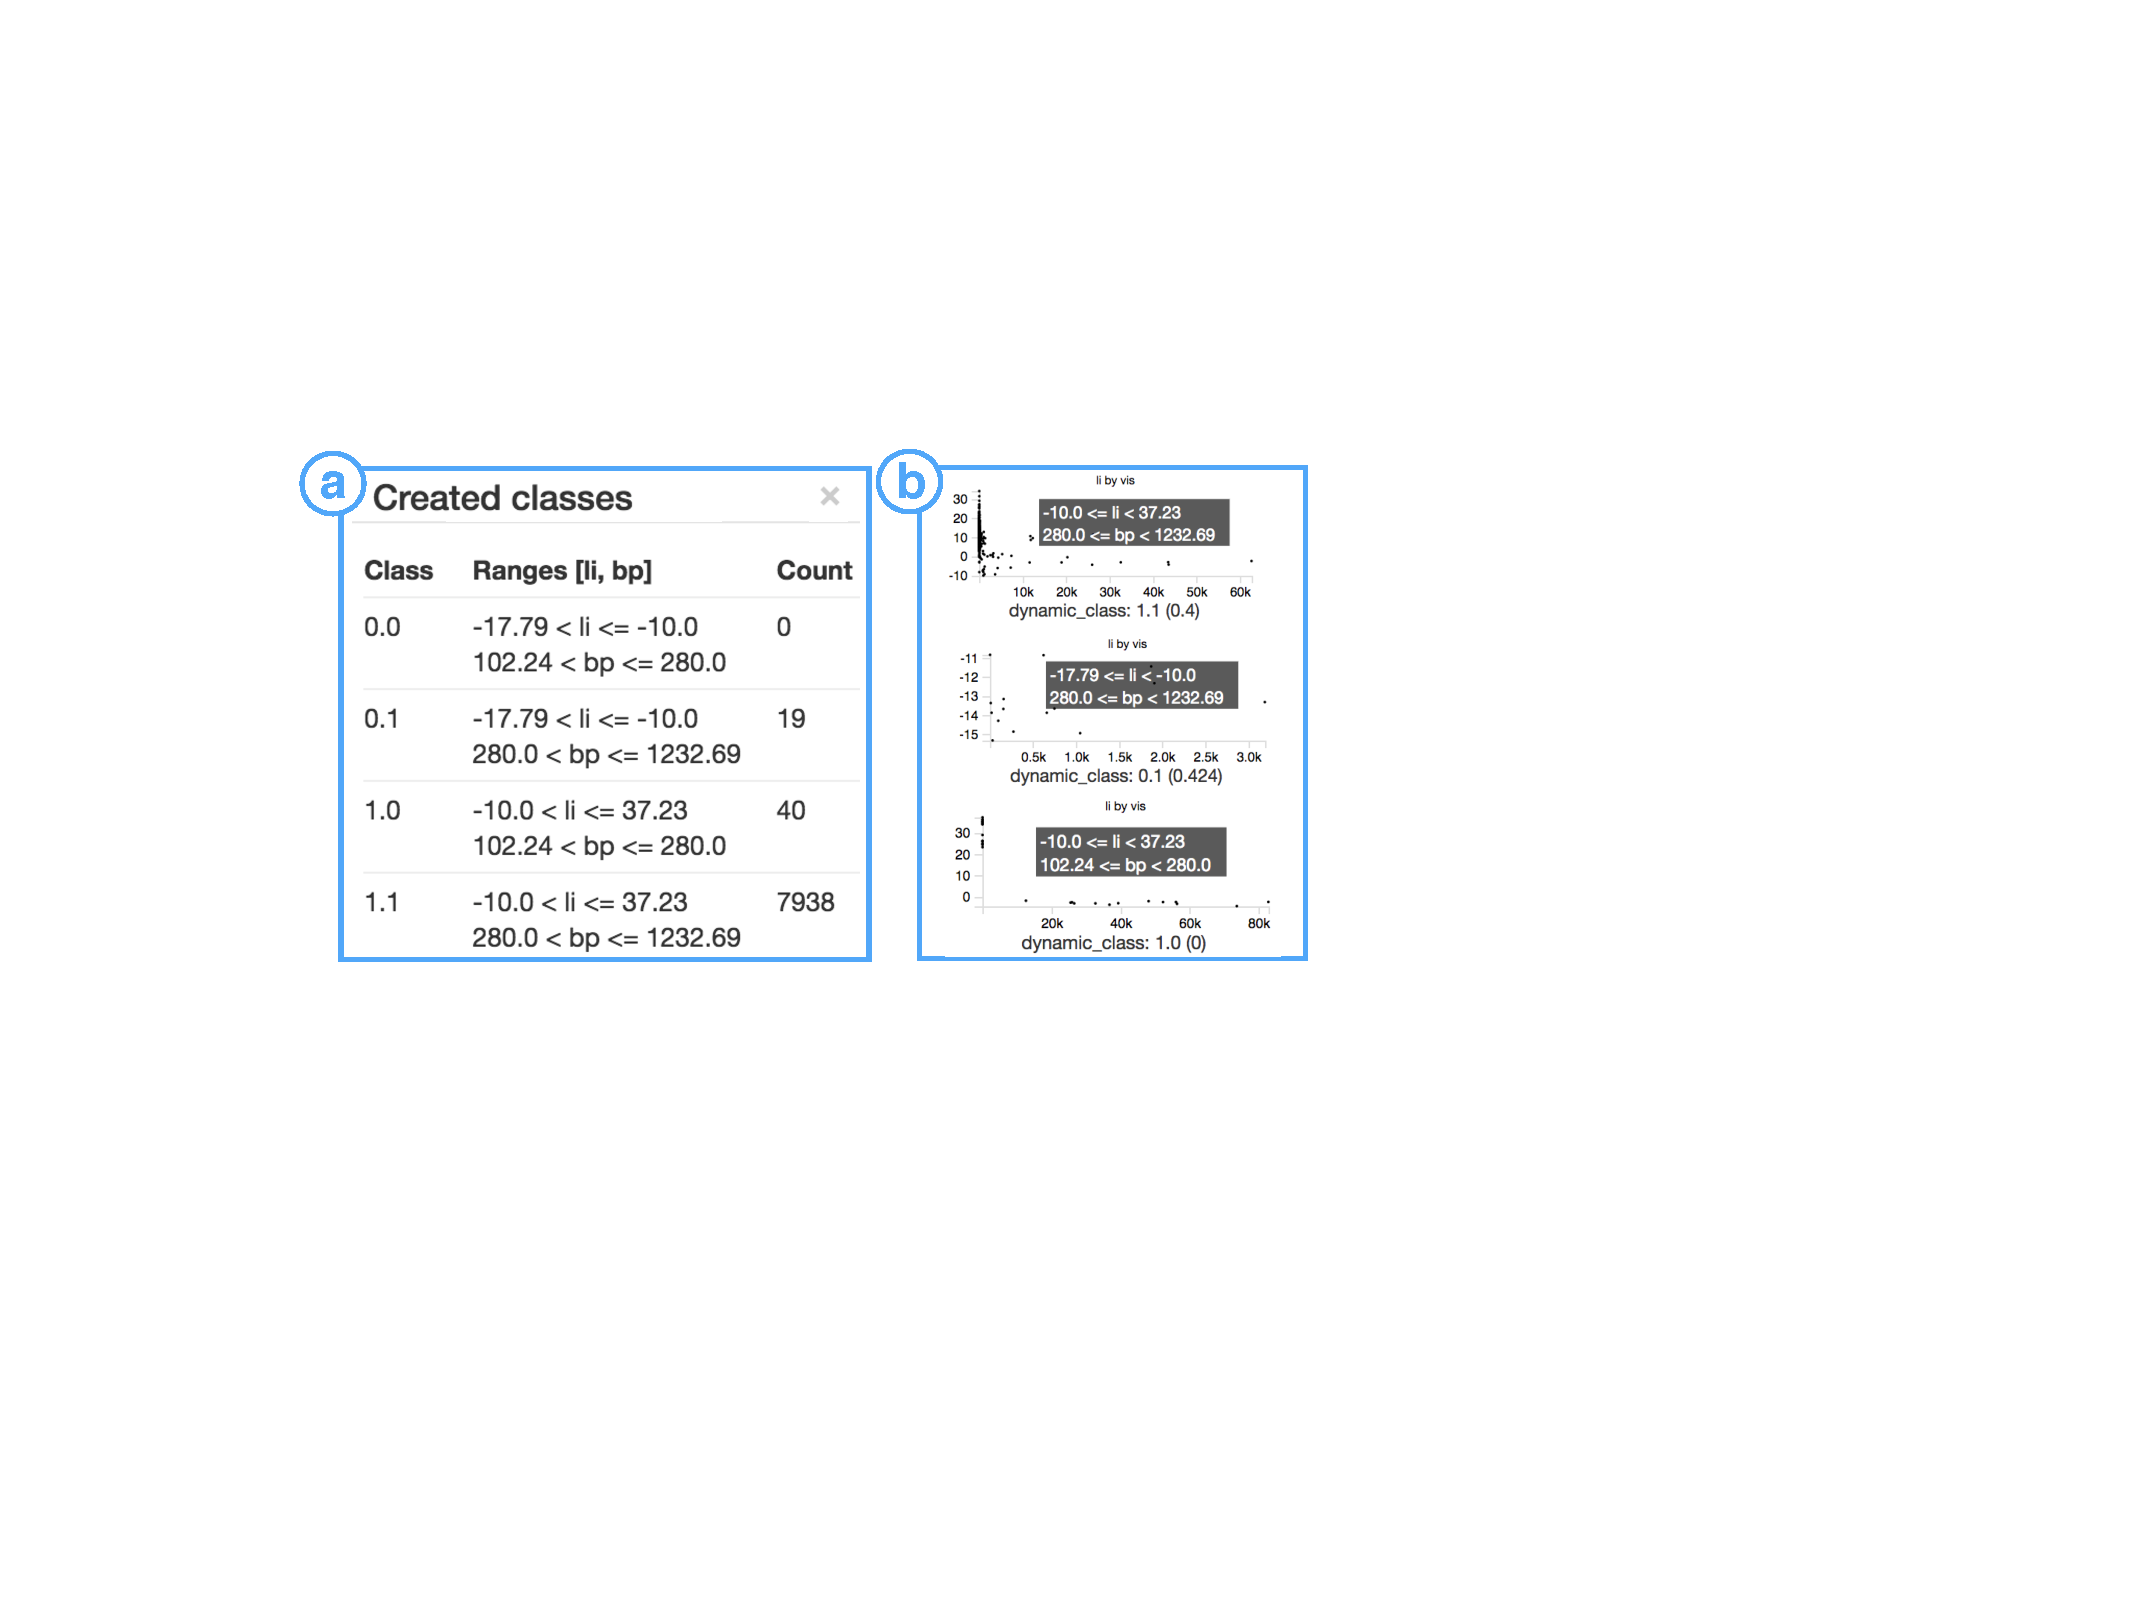
\includegraphics[width=0.95\linewidth]{figures/dcc.pdf}
      \vspace{-6pt}
      \caption{\change{Example of dynamic classes. (a) Four different classes with different Lithium solvation energies (li) and boiling point (bp) attributes based on user-defined data ranges. (b) Users can hover over the visualizations for each dynamic class to see the corresponding attribute ranges for each class. The visualizations of dynamic classes are aggregate across all the visualizations that lie in that class based on the user-selected aggregation method.}}
      \label{dcc}
      \vspace{-10pt}
    \end{figure}
  \enumend
}
%We designed two dynamic faceting features coupled with coordinated views that enabled users to specify subsets of data they are querying on and see immediate changes updated in the query, representative, and outlier results.
%\boldpara{Group Comparison} addresses a common analytical task where users want to
% , as shown in Figure~\ref{dcc}.
%While input equations are useful when simple analytical models exist, this may not be true for other domains. In these scenarios, users can upload a query pattern of a sequence of points
 %Similarly, Google Correlate allows users to upload their own time series or enter search keywords that corresponds to a time series.
%, usually as part of the downstream analysis of the exploratory workflow. %For example, the genetics team are trying to develop a time series prediction algorithm using machine learning based on some biological parameters \cite{Peng2016}.
\change{
  \boldpara{V) Result querying}
  \nstitle{Purpose:} Querying based on the displayed results (either from the ranked list in Figure~\ref{zvOverview}C or recommendations from Figure~\ref{zvOverview}E), essentially requesting for patterns similar to the selected data pattern.
  \problemlist
    \item General need for having to search for a pattern similar to a visualization of interest. For example, G1 was interested in the gene `Esrrb' and wanted to find other genes that exhibits a similar pattern to it.
  \enumend
  \featurelist
    \item In \zvpp, users can drag and drop a visualization in either the results pane or the representative and outliers to the query canvas (Figure \ref{zvOverview}j). Similarly, TimeSearcher enable users to instantiate queries via drag-and-drop, whereas QuerySketch does so through double clicking.
  \enumend
  \boldpara{VI) Recommendation}
  \nstitle{Purpose:} displays visualizations that may be of interest to the users based on the data context.
  \problemlist
    \item Geneticists are often interested in learning about the common gene expression profiles in their dataset.
  \enumend
  \featurelist
    \item \zvpp provides visualizations of representative trends based on clustering and highlights outlier instances\techreport{ that look different from the rest of the visualizations} (Figure \ref{zvOverview}E).%The recommendation feature is unique to \zv, which provides visualizations of representative trends based on clustering and highlights outlier instances that looks different from the rest of the visualizations (Figure \ref{zvOverview}k,l).
  \enumend
}
% In this section, we first describe a model to help characterize the design space for VQS based on the analytical workload and usage patterns from different use cases. Then, we present design challenges related to each of the process.
\begin{table}
		\centering
    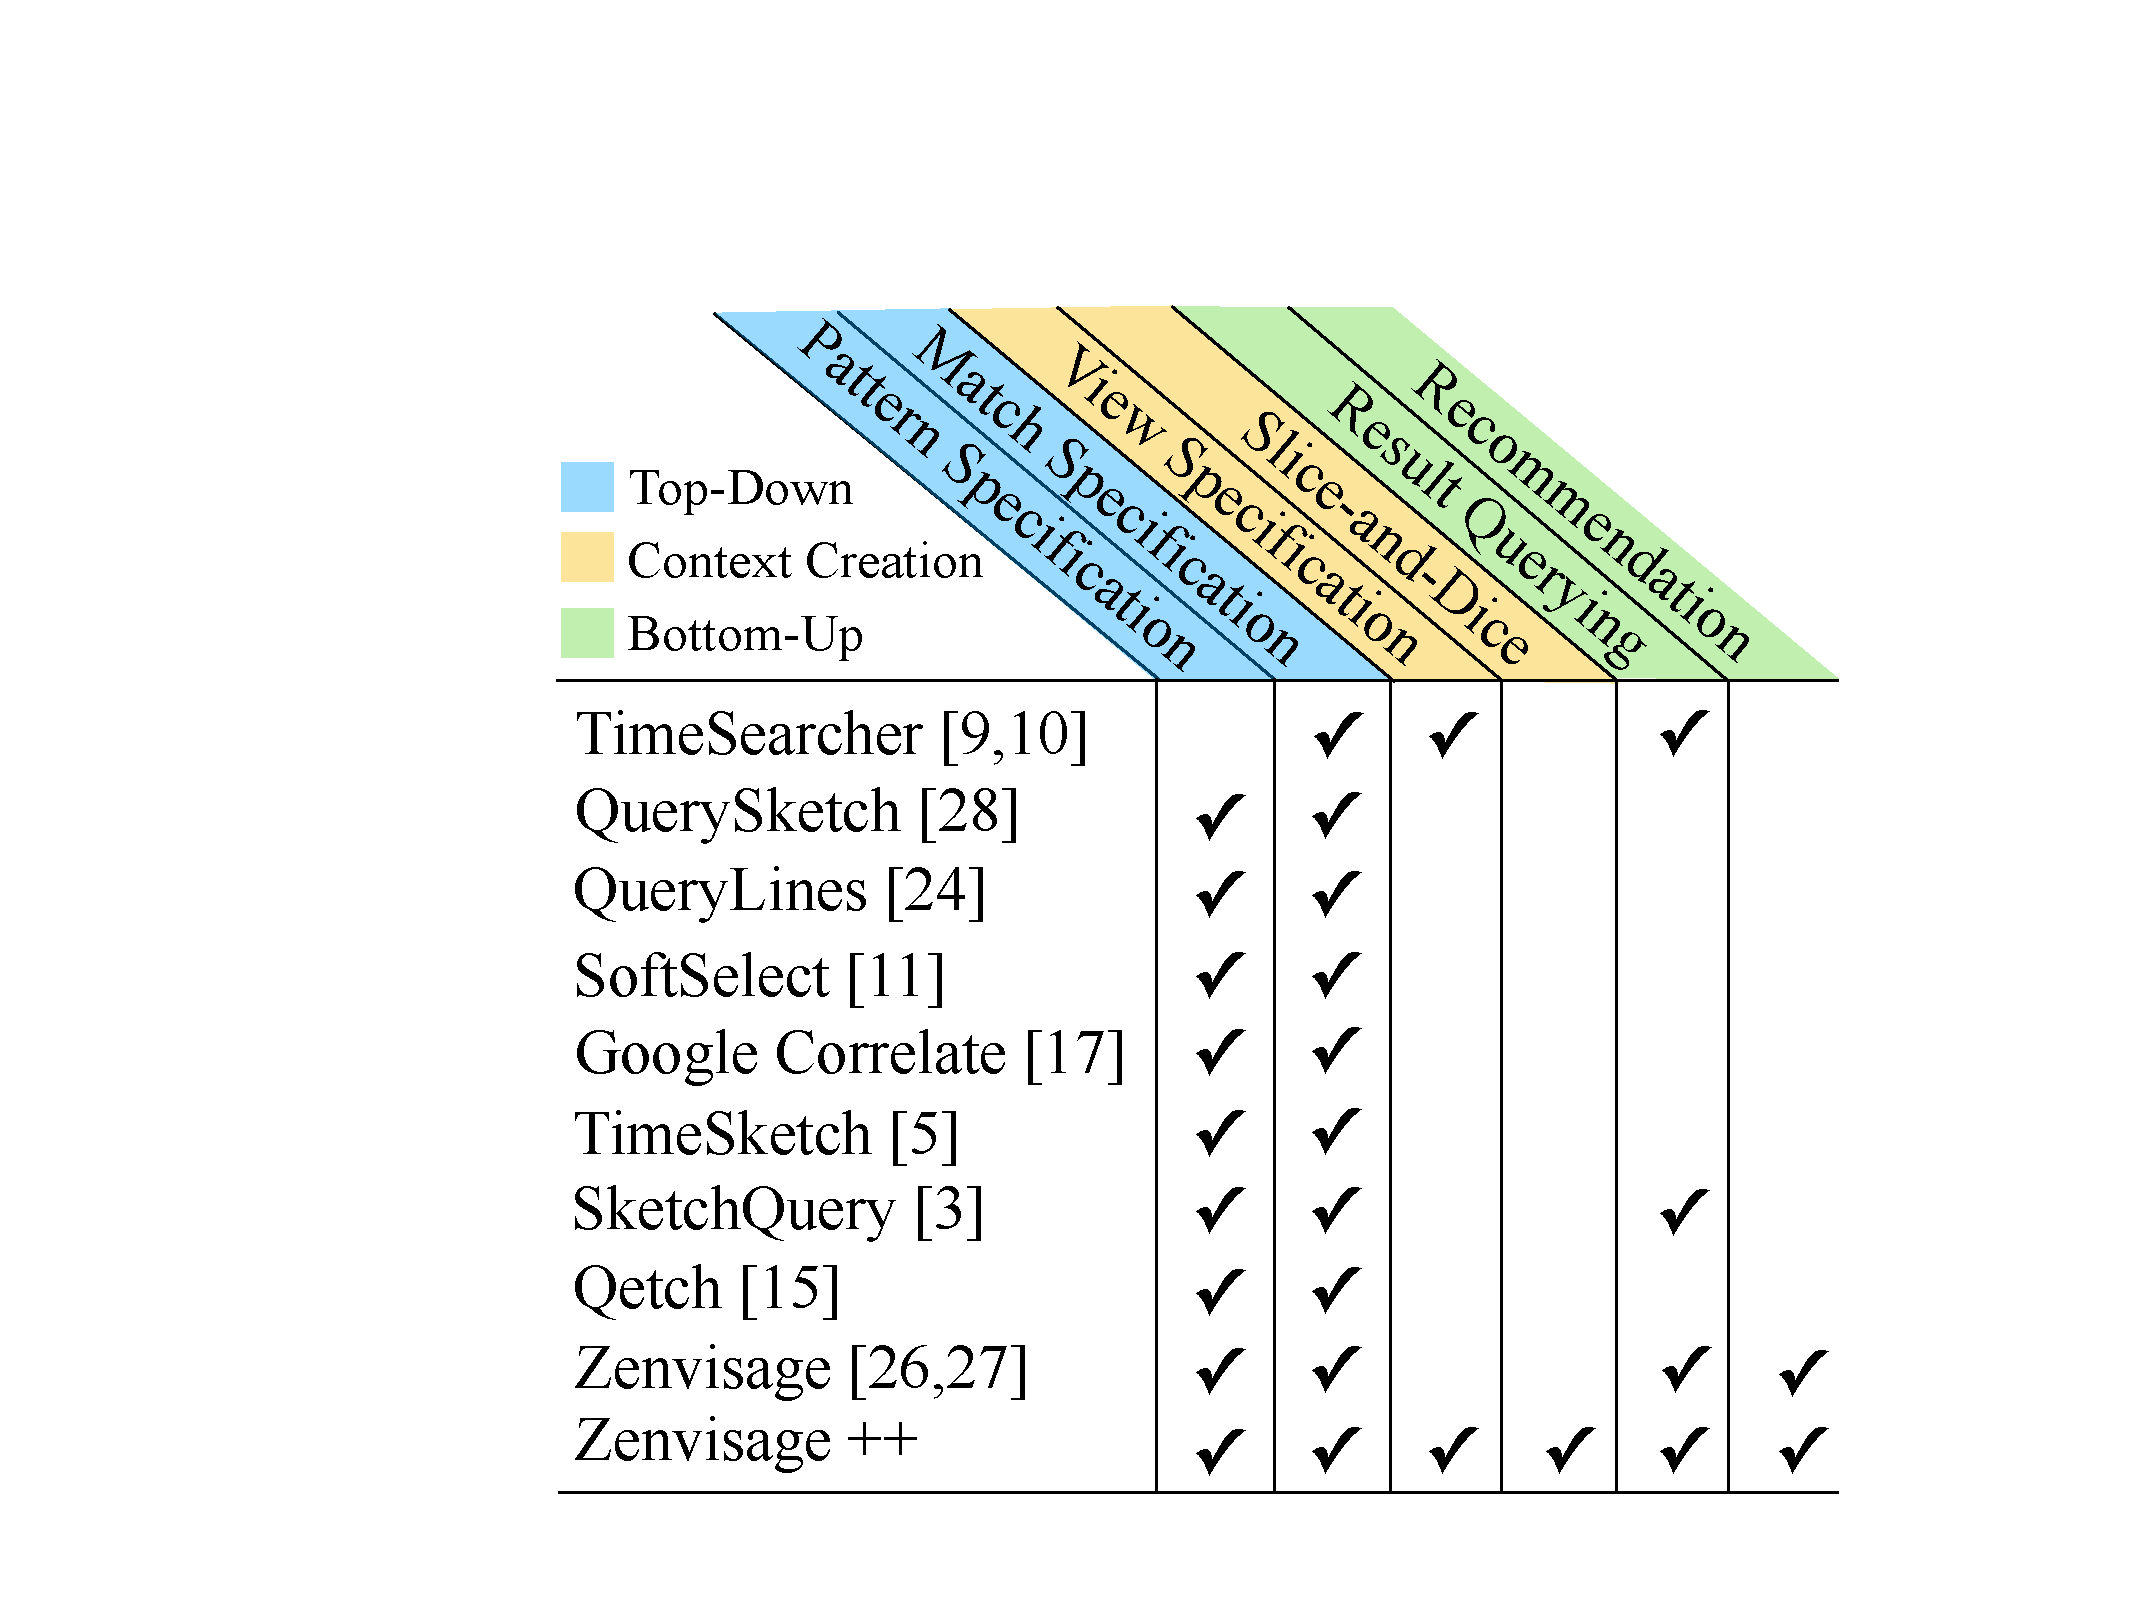
\includegraphics[width=0.8\linewidth]{figures/related_works_table.pdf}
    \caption{Table summarizing whether key \change{functional components} (columns) are covered by past systems (row), indicated by checked cells. Column header colors blue, orange, green represents three sensemaking process (top-down querying, search with context, and bottom-up querying)\cut{ described in Section~\ref{sec:pd_findings}}. The heavily-used, practical features in our study for context-creation and bottom-up inquiry is largely missing from prior VQSs.}
    \label{table:relatedwork}
    \vspace{-10pt}
\end{table}
\begin{figure*}[ht!]
  \centering
  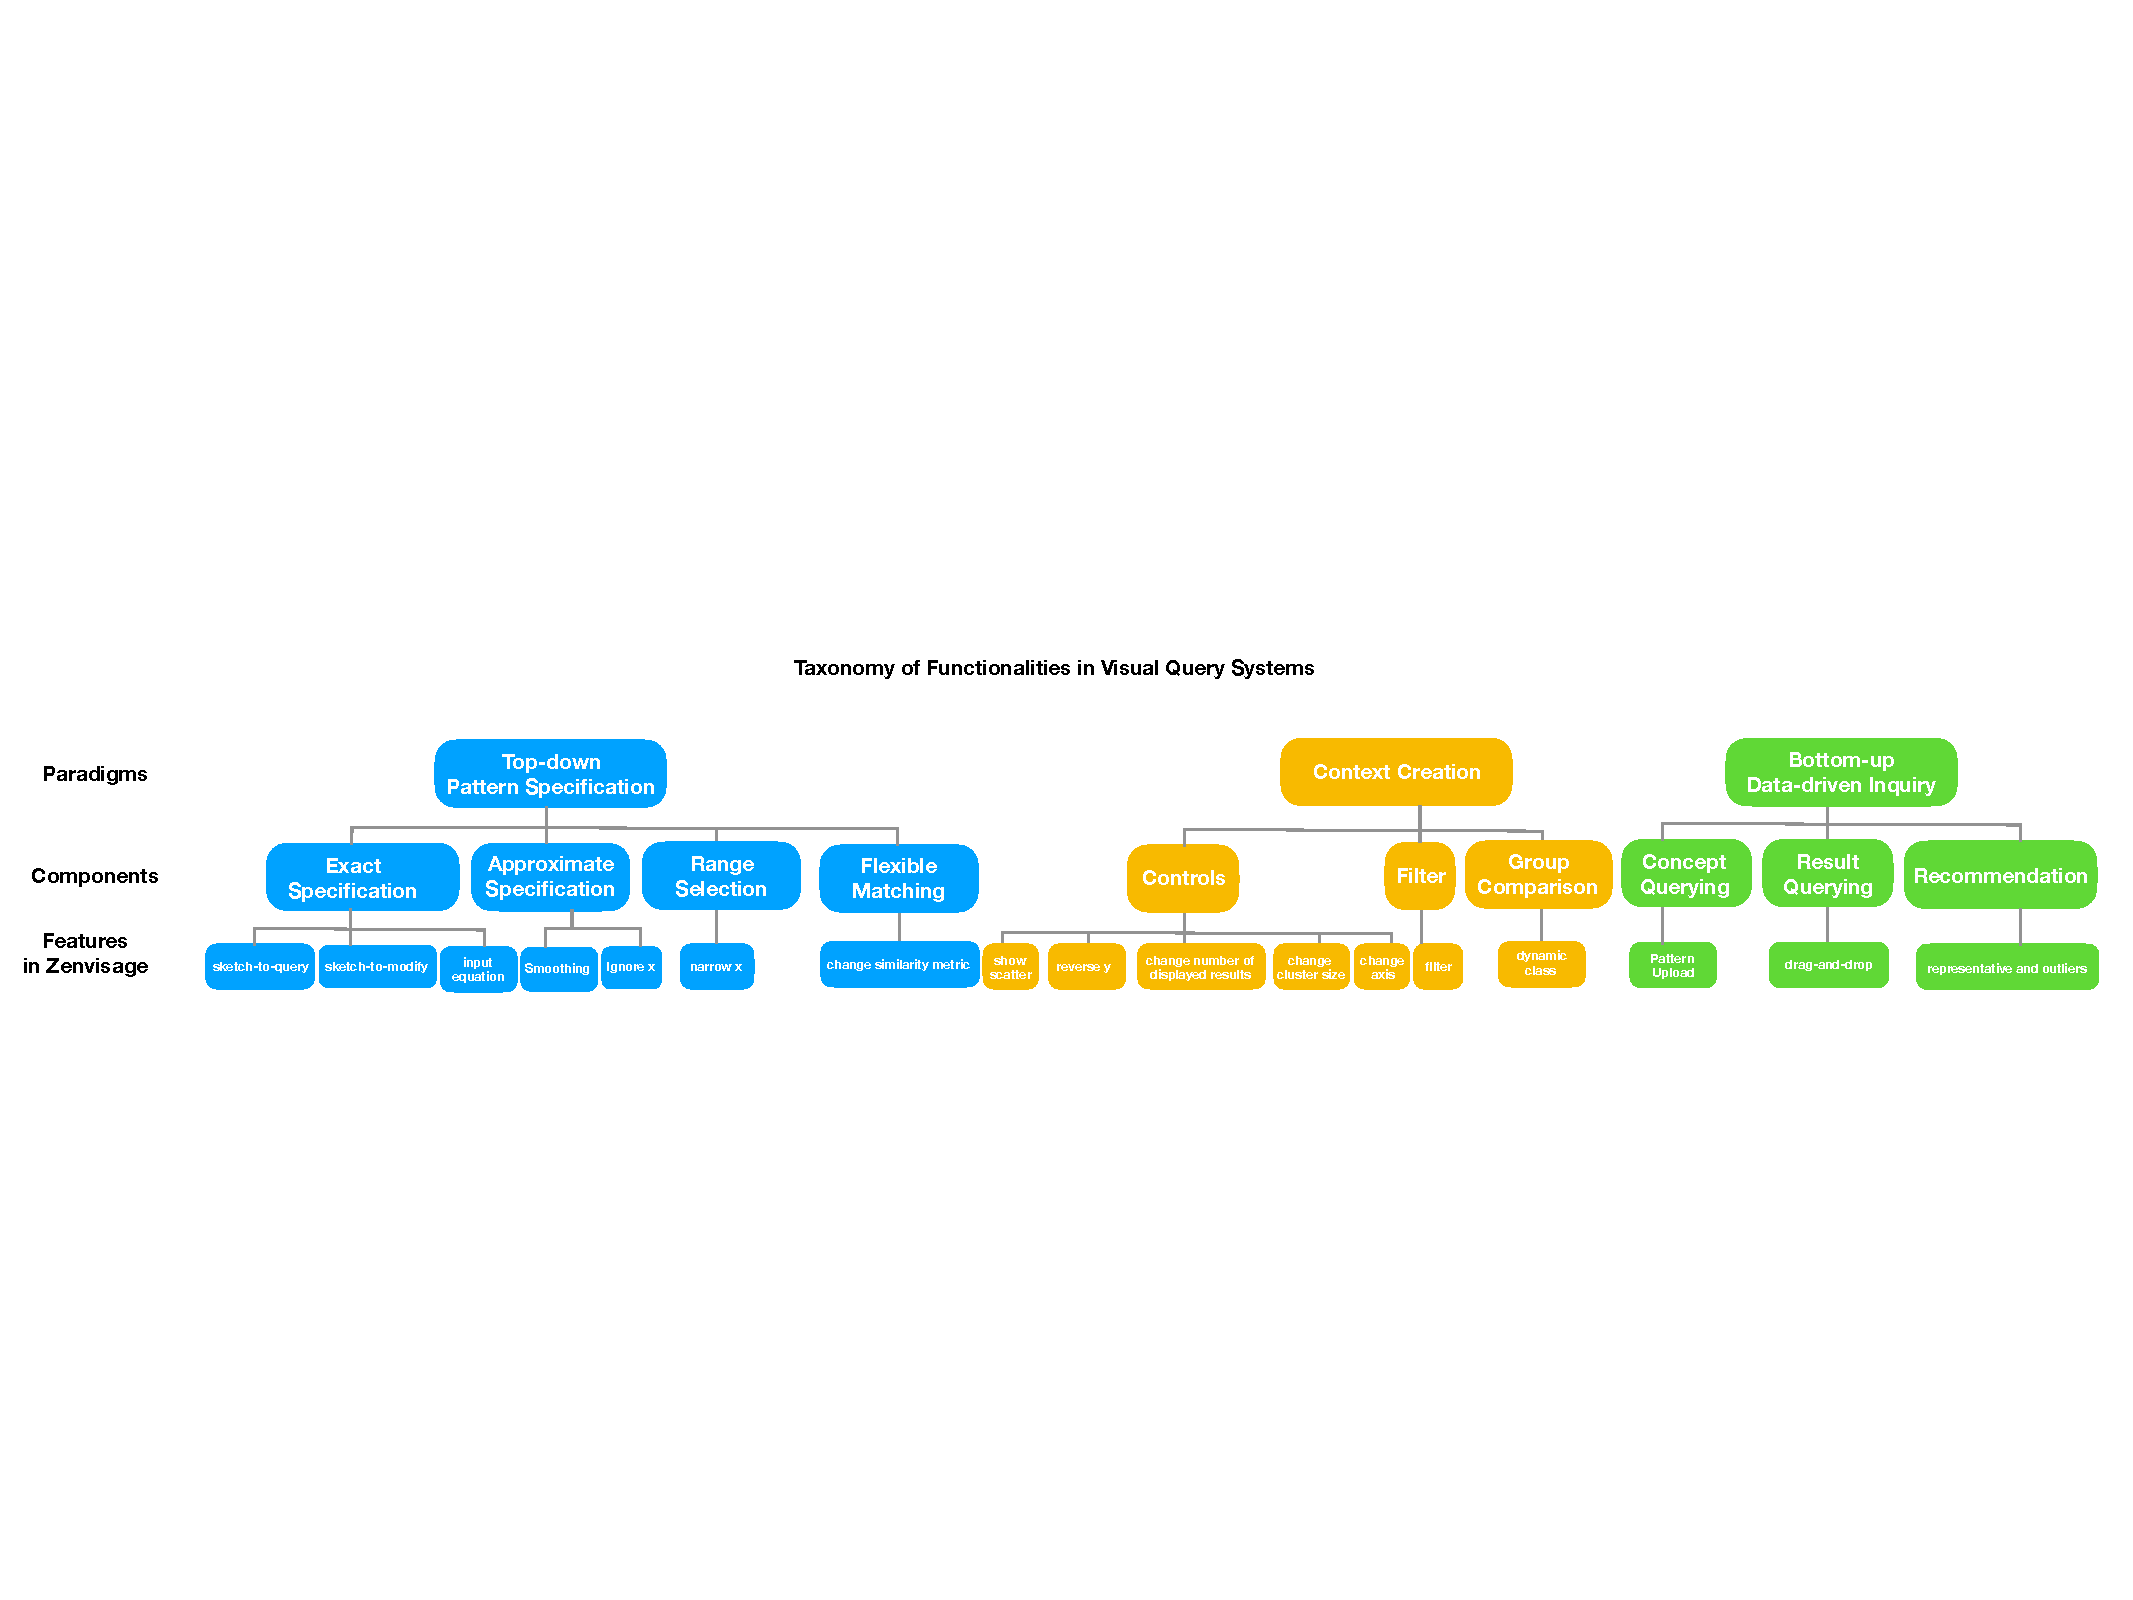
\includegraphics[width=0.9\linewidth]{figures/taxonomy.pdf}
  \caption{Taxonomy of functionalities in VQSs. Each of the three sensemaking process is broken down into key functional components in VQSs. \change{We list the types of questions addressed by each component from a system's perspective.}} %, which is instantiated as features in \zvpp.}% The bottom-most layer connects the use cases features that have practical or envisioned usage based on the evaluation study.}
  \label{fig:taxonomy}
\end{figure*}
}
